\begin{wrapfigure}[0]{r}[-4cm]{3cm}
 \vspace{-6cm}
 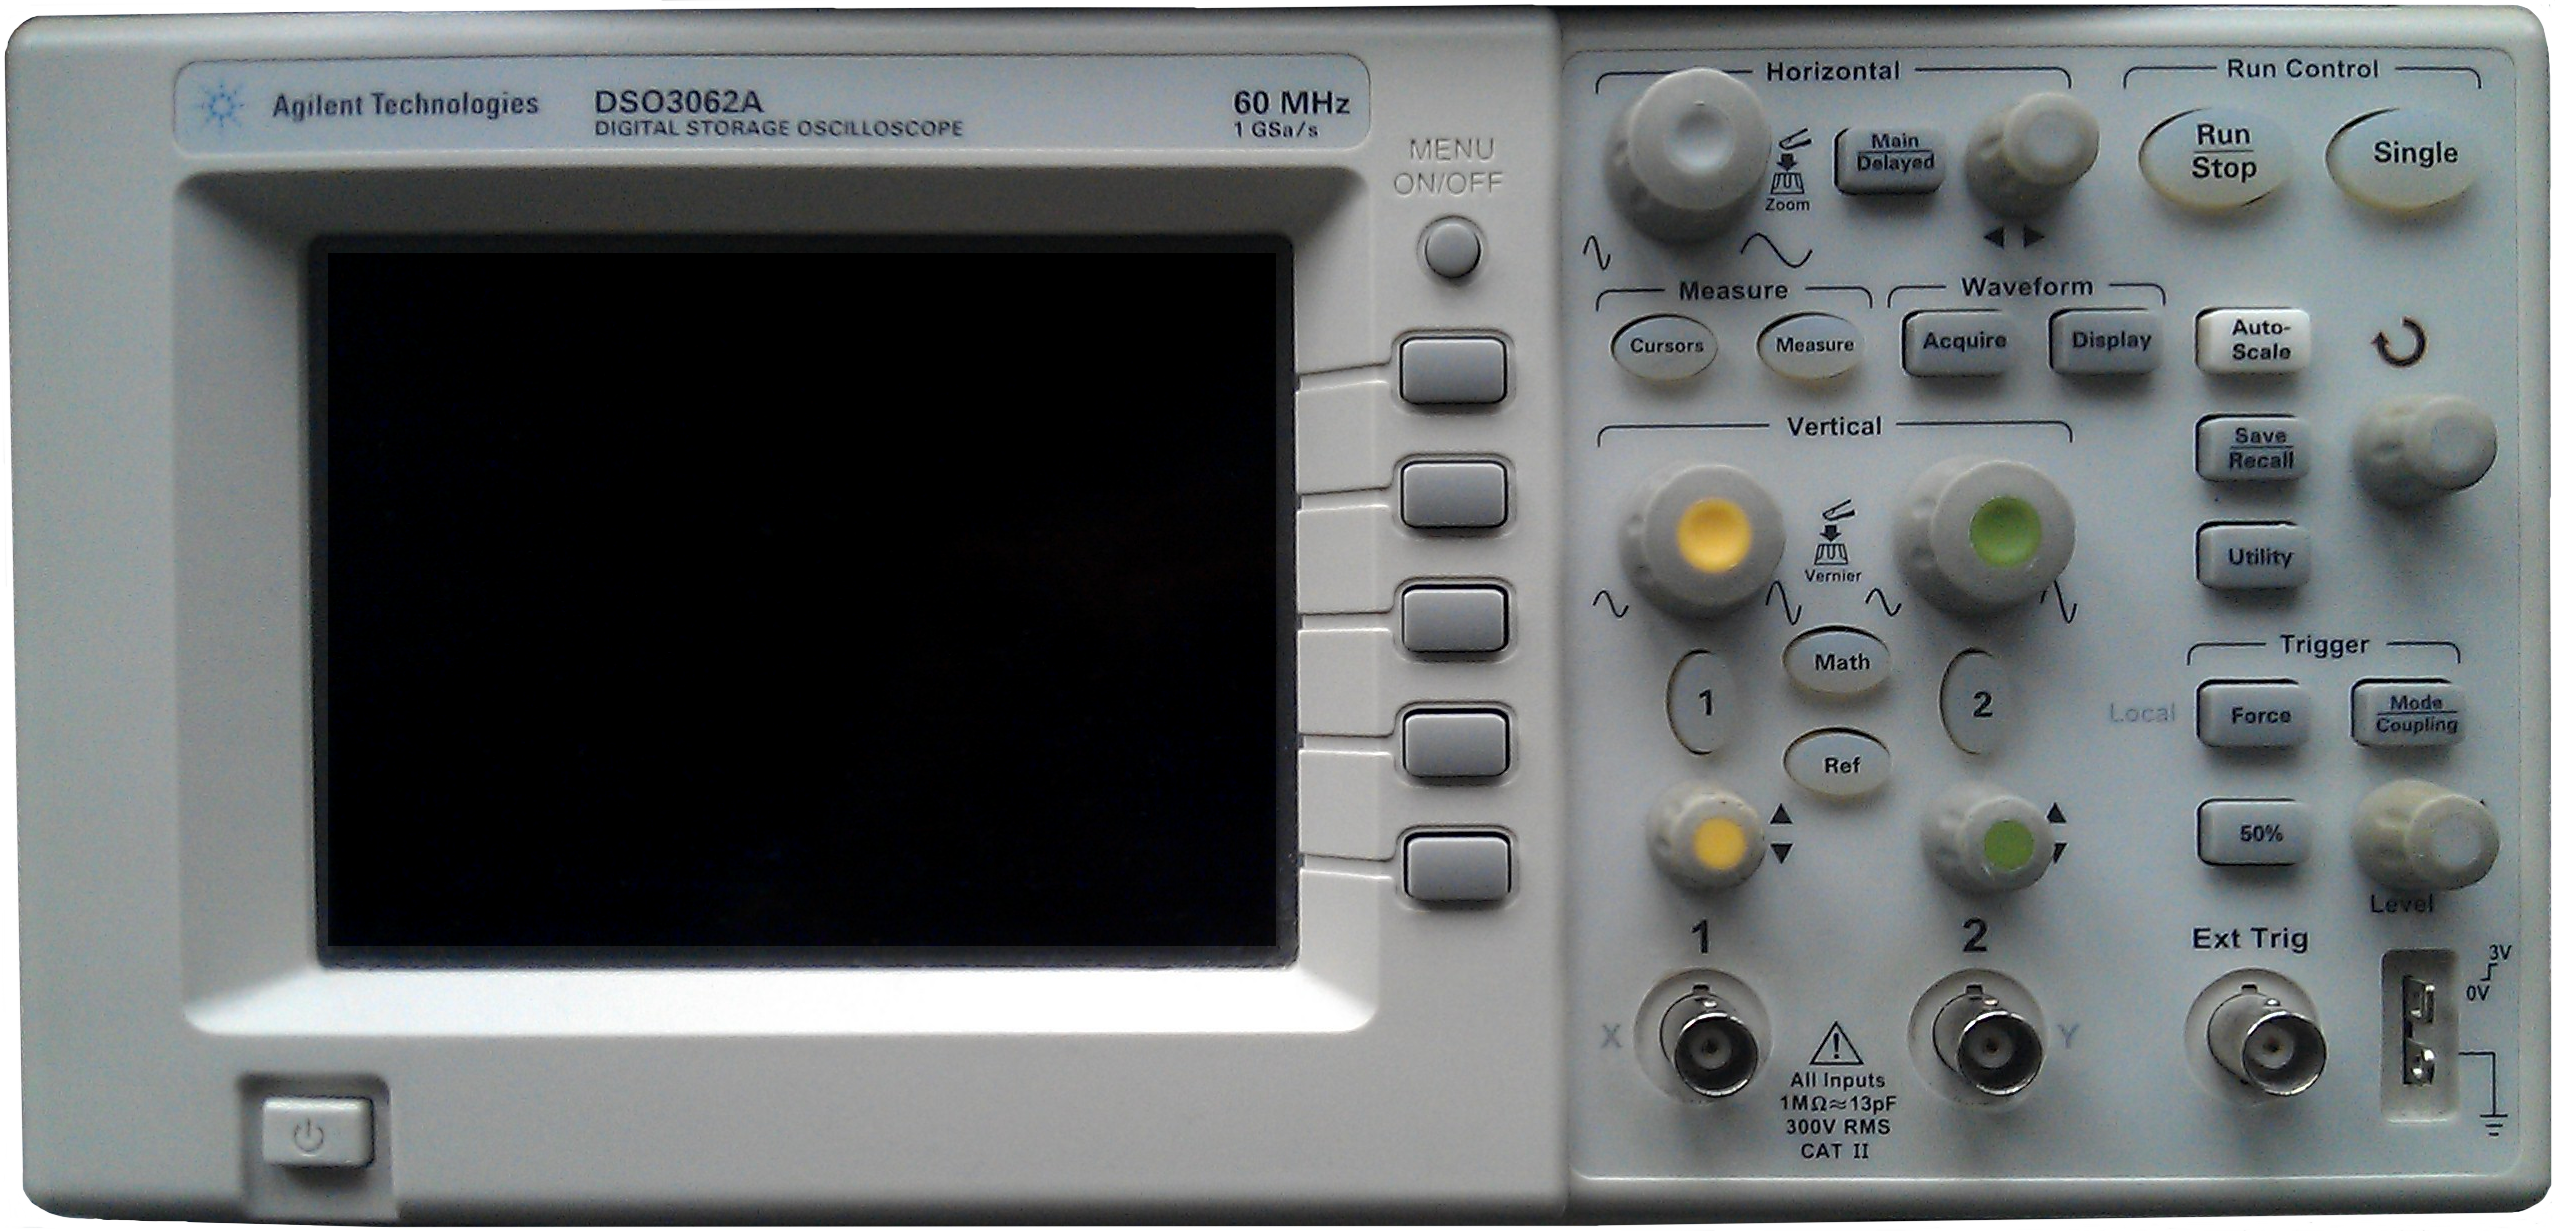
\includegraphics[scale=0.08]{Messtechnik/Bilder/oszi_foto.png}
 \vspace{-6cm}
\end{wrapfigure}

\section*{Theorie- und Prüfungsfragen} 

\mucho{1}{TJ101}
{Das Prinzip des Drespulmessgerätes berut auf}%Frage
{der Wechselwirkung der Kräfte zwischen zwei permanent magnetischen Feldern.}%A
{der Wechselwirkung der Kräfte zwischen einem magnetischen und einem elektrischen Feld.}%B
{der Wechselwirkung der Kräfte zwischen einem permanent magnetischen und einem elektromagentischen Feld.}%C
{dem erdmagentischen Feld.}%D
{C}%Lösung

\mucho{2}{TJ111}
{Mit welchem Strom zeigt ein 20-$k\Omega/V$-Instrument Vollausschlag?}%Frage
{500$\mu A$}%A
{5$mA$}%B
{50$mA$}%C
{50$\mu A$}%D
{D}%Lösung

\mucho{3}{TJ102}
{Das Drehspulmesswerk in der folgenden Schaltung hat einen maximalen Messstrom $I_M = 100\mu A$ und einen Messwerkwiderstand $R_M = 1 k\Omega$.}%Frage
{10V}%A
{50V}%B
{500V}%C
{100V}%D
{B}%Lösung


\mucho{4}{TJ805}
{Mit einem Voltmeter der Klasse 1.5, das einen Skalenendwert von 300V hat, messen Sie an einer Spannungsquelle 230V. In welchem Bereich liegt der wahre Wert?}%Frage
{Er liegt zwischen 225,5 und 234,5V.}%A
{Er liegt zwischen 226,5 und 233,5V.}%B
{Er liegt zwischen 229,5 und 230,5V.}%C
{Er liegt zwischen 229,7 und 230,3V.}%D
{A}%Lösung


\mucho{5}{TJ115}
{Ein Drehspulmessgerät hat normalerweise eine Genauigkeit von}%Frage
{ca. 1,5 \% vom Endausschlag.}%A
{ca. 0,3 \% vom Ablesewert.}%B
{ca. 0,3 \% vom Endausschlag.}%C
{ca. 0,05 \% vom Ablesewert.}%D
{A}%Lösung

\mucho{6}{TG219}
{Die richtige Oberwellenauswahl in einer Vervielfachungsstufe lässt sich am leichtesten mit einem}%Frage
{Diodentastkopf prüfen.}%A
{Absorptionsfrequenzmesser prüfen.}%B
{Universalmessgerät prüfen.}%C
{Frequenzzähler prüfen.}%D
{B}%Lösung


\mucho{7}{TJ602}
{Ein Absorptionsfrequenzmesser hat normalerweise eine Genauigkeit von}%Frage
{1 \%.}%A
{5 \%. }%B
{0,05 \%.}%C
{0,001 \%.}%D
{B}%Lösung


\mucho{8}{TJ812}
{Wie ermittelt man die Resonanzfrequenz eines passiven Schwingkreises?}%Frage
{Durch Messung von L und C und Berechnung oder z.B. mit einem Dip-Meter.}%A
{Mit einem Frequenzmesser oder einem Oszilloskop.}%B
{Mit einem Digital-Multimeter in der Stellung Frequenzmessung.}%C
{Mit Hilfe der S-Meter Anzeige bei Anschluss des Schwingkreises an den Empfängereingang.}%D
{A}%Lösung

\mucho{9}{TJ206}
{Ein Dip-Meter hat normalerweise eine Genauigkeit von etwa}%Frage
{1 \%.}%A
{10 \%.}%B
{0,05 \%.}%C
{0,001 \%.}%D
{B}%Lösung

\mucho{9}{TJ501}
{Um die Skalenendwerte einer Sende-/Empfangsanlage mit VFO mit hinreichender Genauigkeit zu überprüfen, kann man}%Frage
{einen Frequenzzähler verwenden.}%A
{ein Dipmeter verwenden.}%B
{einen Absorptionsfrequenzmesser verwenden.}%C
{ein Oszilloskop verwenden.}%D
{A}%Lösung

\mucho{10}{TJ402}
{Für welchen Zweck wird eine Stehwellenmessbrücke verwendet?}%Frage
{Zur Überprüfung der Anpassung des Senders an die Antenne}%A
{zur Frequenzkontrolle.}%B
{zur Modulationskontrolle.}%C
{als Abschluss des Senders.}%D
{A}%Lösung

\mucho{11}{TJ305}
{Welches dieser Geräte wird für die Anzeige von NF-Verzerrungen verwendet?}%Frage
{Frequenzzähler}%A
{Transistorvoltmeter}%B
{Vielfachmessgerät}%C
{Oszilloskop}%D
{D}%Lösung

\mucho{12}{TJ303}
{Um auf dem Bildschirm eines Oszilloskops ein stehendes Bild statt durchlaufender Wellenzüge zu erhalten muss, das Oszilloskop}%Frage
{eine Triggereinrichtung haben.}%A
{einen X-Vorteiler haben.}%B
{einen Y-Vorteiler haben. \vspace*{-0.06cm}}%C
{einen Frequenzmarken-Generator haben.}%D
{A}%Lösung
